\documentclass[a4paper]{article}

%% Language and font encodings
\usepackage[english]{babel}
\usepackage[utf8x]{inputenc}
\usepackage[T1]{fontenc}

%% Sets page size and margins
\usepackage[a4paper,top=3cm,bottom=2cm,left=3cm,right=3cm,marginparwidth=1.75cm]{geometry}

%% Useful packages
\usepackage{amsmath}
\usepackage{graphicx}
\usepackage[colorinlistoftodos]{todonotes}
\usepackage[colorlinks=true, allcolors=blue]{hyperref}
\usepackage{alltt}

\title{Reporte de Actividad 9}
\author{Valenzuela Terán Jonás}

\begin{document}
\maketitle


\begin{center}

	
\includegraphics[height=5cm]{wxmaxima.png}

\end{center}

\section{Introducción}

Maxima es un sistema de álgebra computacional (CAS), es software libre basado en Macsyma. Contiene herramientas para resolver problemas simbólicos, numéricos y gráficos. Esto ayuda a concentrar el trabajo matemático en la computadora, como una calculadora extendida. wxMaxima es la interface gráfica de Maxima, que requiere de menos memorización de comandos, y hace trabajar con el más fácil y accesible para usuarios con menos experiencia en esa categoría de programas, además, ofrece ciertas notaciones matemáticas. Maxima es una aplicación de comandos de linea, de entrada y salida, cabe notar que es sensible a mayúsculas.


\section{Manual de introductorio de \textit{wxmaxima}}

\subsection{Operaciones}

Para ejecutar una operación, se presiona SHIFT+ENTER, se agrega ; para mostrar el resultado de la operación, se agrega \$ para no mostrar la salida.

Sintaxis de operaciones basicas:
Suma: a + b
Resta: a - b
Multiplicación: a * b
División: a / b
Potencia: a\^b
Raíz: sqrt(a)

Podemos usar salidas anteriores en las operaciones usando \%, o \%o1 donde 1 hace referencia a la salida 1 del código.

Un ejemplo:

\begin{alltt}
sqrt(a + b);
$\%$ * c;
\end{alltt}

Para mostrar la aproximación decimal de un numero irracional o una fracción como $\frac{1}{3}$:

\begin{alltt}
1 / 3
float(\%)
\end{alltt}


\subsection{Definir variables y funciones}
Se escribe el nombre de la variable, seguida de 2 puntos y su valor asignado:

\begin{alltt}
base: 10 \$
altura: 5 \$
area: base * altura / 2
\end{alltt}

Ahora vemos como definimos y evaluamos una función:

\begin{alltt}
f(x) := x^2 + a \$
f(5), a = -5;
\end{alltt}

\subsection{Operaciones especiales}

Es posible hacer muchas más cosas que una calculadora convencional, por ejemplo, integración indefinida y definida respectivamente:

\begin{alltt}
integrate( x^2, x);
integrate( 1/x, x, 0, \% pi);
\end{alltt}

Primero se agrega la función a integrar, luego con respecto a la variable se integrara, y después, opcional mente, los límites de integración. También es posible brindar información a Maxima usando la función \textit{assume}: 

\begin{alltt}
assume(a > 0)\$
integrate((1+x^2)/a,x);
forget(a > 0)
\end{alltt}

Así como encontrar las soluciones de una ecuación::

\begin{alltt}
solve(a*x^2 + b*x^2 + c = 0,x);
\end{alltt}

Maxima cuenta con herramientas de álgebra lineal, para crear y operar con una matriz, observemos los ejemplos:

\begin{verbatim}
A: matrix([1,-1],
		          [1,sin(c)]);
B: invert(A);
\end{verbatim}

Al igual que otras herramientas de computo simbólico,¡maxima puede derivar usando la regla de la cadena y resolver ecuaciones diferenciales ordinarias!

\begin{alltt}
f(x) := x^2 \$
diff(f(x),x);
g(y) := sin(y) \$
diff( g(f(x)) , x)
\end{alltt}


\begin{alltt}
y''(t) + w^2 = y(t) = 0
assume(omega >0);
ode2('diff(y,t,2) + w^2 * y = 0, y, t );
ic2(\%, t=0, y=amp, 'diff(y,t) = 0;
\end{alltt}

Finalmente, mostraremos como crear gráficas 2D y 3D, usando parametrización en 2D y función explícita en 3D:

\begin{alltt}
wxplot2d([sin(x), cos(x)], [x,0,2*\% pi]);
wxplot3d( exp(-x^2 - y^2), [x,-2,2],[y,-2,2]);
\end{alltt}

Existen muchas más herramientas en wxmaxima, útiles para problemas más específicos como estadística, todo esto puede accederse a través de la interface que ofrece wxmaxima.


\section{Ejemplo resuelto: }

Cubriremos más a fondo la utilidad de máxima enfocándonos en integrales mientras resolvemos un problema:

\subsection{Problema: Calculo de volumen con integrales triples}

Bosqueje y calcule el volumen del sólido $\Omega$, descrito bajo el paraboloide $z = 3x^2 +y^2$, y arriba de la región acotada por $y=x$, y $x=y^2 - y$.

\subsection{Solución}

Para resolver casi cualquier problema, es importante visualizarlo primero, en este caso, para definir los límites de la triple integral con $f(x,y,z)=1$ que calcula el volumen de la región de integración:

\begin{center}
$\int \int \int_\Omega f(x,y,z) dV = \int \int \int_\Omega dV = Vol(\Omega)$
\end{center}

Realizamos la gráfica con el comando \textit{wxplot3d} lo que acota la altura:

\begin{verbatim}
wxplot3d(3*x^2+y^2,[x,-5,5],[y,-5,5]);
\end{verbatim}

\begin{center}
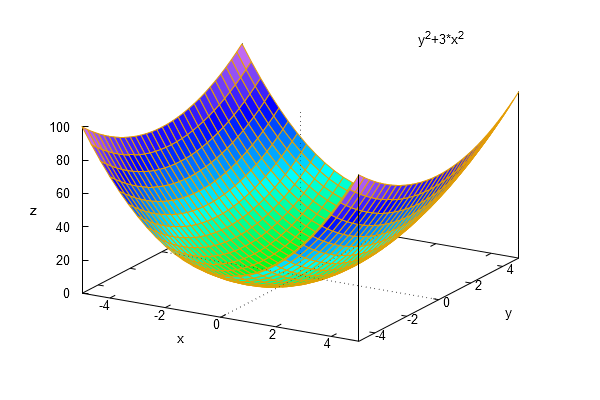
\includegraphics[height=6.5cm]{rep9_1_.png}
\end{center}

Ahora graficamos la región del plano xy que acota al sólido:

\begin{verbatim}
wxplot2d(x,[x,-5,5]);
wxplot2d(x^2-x,[x,-5,5]); /* Donde x es y y viceversa */
\end{verbatim}

\begin{center}
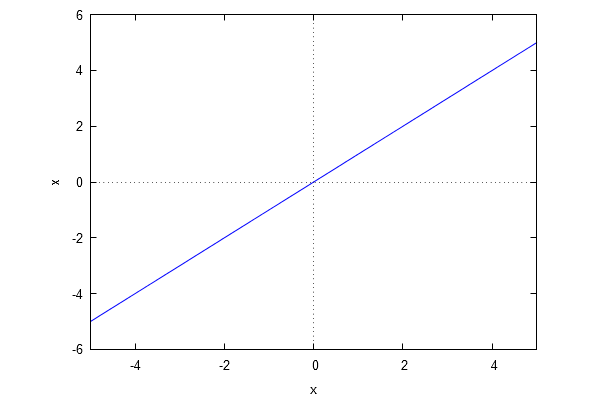
\includegraphics[height=6.5cm]{rep9_2.png}

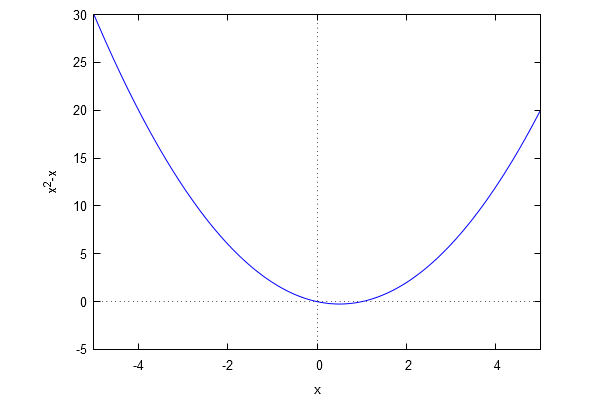
\includegraphics[height=6.5cm]{rep9_3.png}
\end{center}

Para definir los límites del plano xy, necesitamos conocer los puntos críticos entre $y=x$ y $x=y^2-y$:

\begin{verbatim}
solve(x-x^2+x=0)
\end{verbatim}

Esto nos da como resultado $x=0$ y $x=2$. Ahora, consideramos los límites de $\Omega$:

\begin{center}
$\displaystyle \int^{2}_{0} \int^{y}_{y^2 -y} \int^{3x^2 +y^2}_{0} dz dx dy = Vol(\Omega)$
\end{center}

Resolvemos analíticamente con la función \textit{integrate} de wxmaxima, integral por integral:

\begin{verbatim}
integrate(1,z,0,3*x^2+y^2)
\end{verbatim}

Nos da la salída $y^2 + 3x^2$, seguimos con la segunda integral

\begin{verbatim}
integrate(%,x,y^2-y,y)
\end{verbatim}

Resulta en $-y^6 +3y^5 -4y^4 +4y^3$, y la tercera:

\begin{verbatim}
integrate(%o15,y,0,2)
\end{verbatim}

Que nos da el resultado $Vol(\Omega) = \frac{144}{35}$.

Como vemos, wxmaxima fue de gran ayuda en los cálculos y procedimientos que requieren de más tiempo, lo que nos permitió enfocarnos en la interpretación del problema, ahorrando tiempo, y disminuyendo margen de error, además, ¡se obtuvieron bosquejos  inigualables!.

\section{Referencias}

\begin{itemize}
\item Documentación de wxmaxima: \textit{http://andrejv.github.io/wxmaxima/help.html}

\item Maxima Tutorial: \textit{https://def.fe.up.pt/dynamics/maxima\_tutorial.html}

\item Derivadas e integrales: \textit{http://webs.um.es/mira/maxima/DerivadasIntegrales.html}
\end{itemize}



\section{Apéndice}
\begin{itemize}
\item     ¿Cuál fue tu primera impresión de wxmaxima?

Es muy buena herramienta, en especial porque es la versión gráfica y fácil de aprender de \textit{maxima}. Además, está muy completa.

\item     ¿Crees que esta herramienta puede ser útil en otros de tus cursos?

Si, ya que la física trata casi cualquier situación con ecuaciones y gráficas, quita buena parte del trabajo matemático para concentrarnos en lo físico.

\item     ¿Qué se te dificultó mas en esta actividad?

Adaptar los problemas al formato que maxima pueda resolver fácilmente y ordenadamente.

\item     ¿Se te hizo compleja esta actividad? ¿Cómo la mejorarías?

No, opino que fue bueno que la actividad se concentrara en la introducción del programa para familiarizarnos con el.

\end{itemize}


\end{document}